\subsection{Video life cycle}
\begin{frame}[fragile]	
	\frametitle{Video life cycle}
	\begin{figure}[!t]
		\centering
		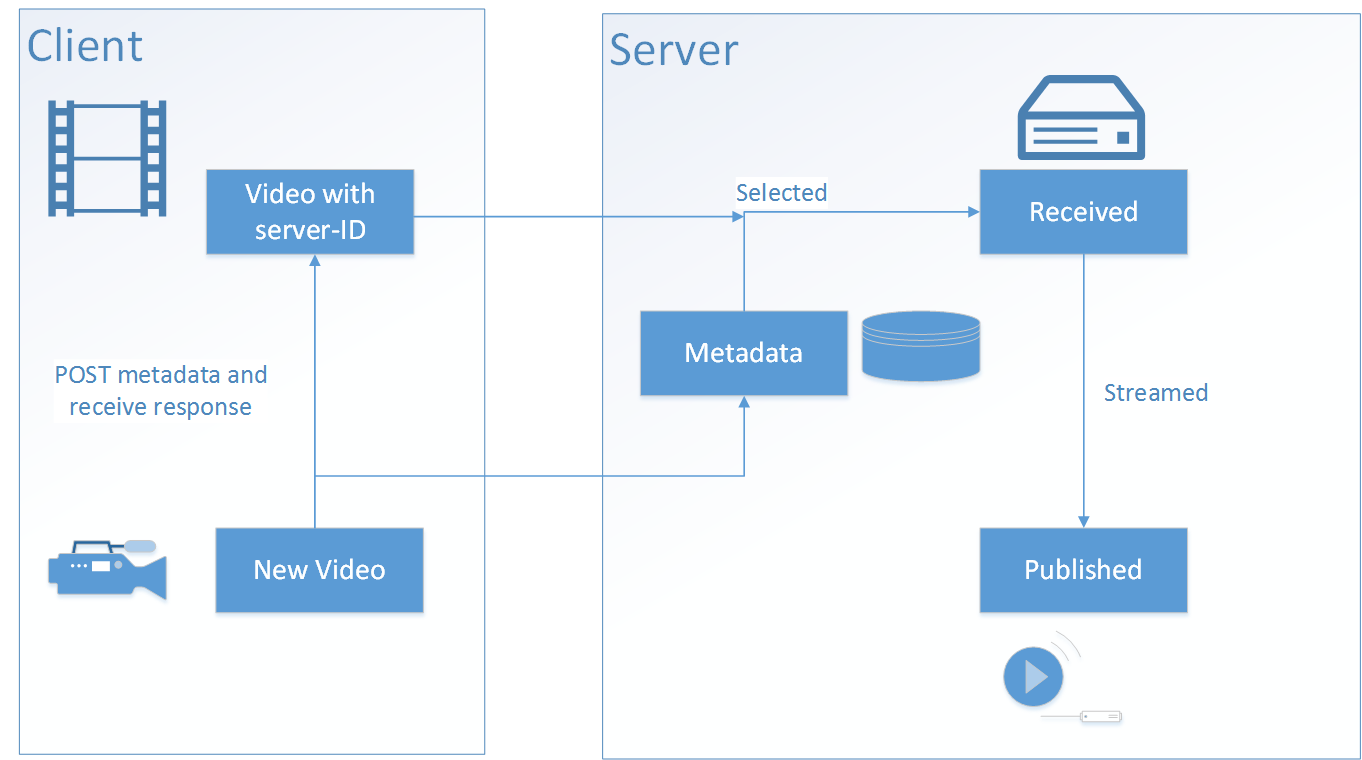
\includegraphics[width=\textwidth,height=\textheight,keepaspectratio]{video_states.png}
		\label{fig:states}
	\end{figure}
\end{frame}

\subsection{Selection algorithm}
\begin{frame}	
	\frametitle{Selection algorithm}
	\texttt{VideoRating} class assignes rank on metadata arrival
	Sigmoid transformation: $\forall x \in [shake, tilt]$
	\begin{align*}
		xs &= \cfrac{x^2}{15 * duration} \\
		f  &= \left(\cfrac{xs}{1+|xs|}\right)^3 &f  &\in [-1, 1] \\
		fn &= \cfrac{f + 1}{2}                  &fn &\in [0, 1]
	\end{align*}
	$$rating = 100 * \sqrt{ \sum\limits_{i \in sensors}{w_i m_i^2} },\ w_{shake} = 0.6,\ w_{tilt} = 0.4$$
	Selection process:
	\begin{itemize}
		\item Only videos starting after the last selected video ends are considered.
		\item Top-rated video is selected for upload
	\end{itemize}
\end{frame}

\begin{frame}	
	\frametitle{Selection algorithm (continued)}
	\begin{figure}[!t]
		\centering
		\subfloat[Scaling]{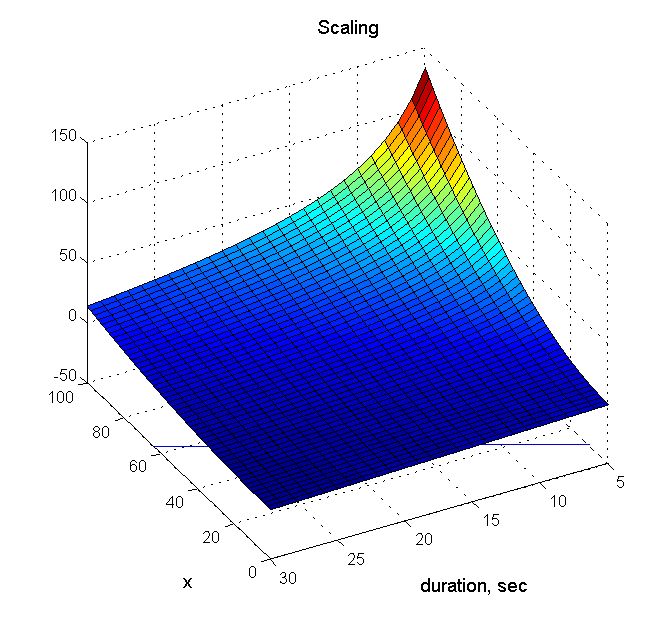
\includegraphics
			[width=.49\textwidth,height=.9\textheight,keepaspectratio]
			{scaling.png}%
			\label{fig:scaling}}
		\hfill
		\subfloat[Sigmoid transformation]{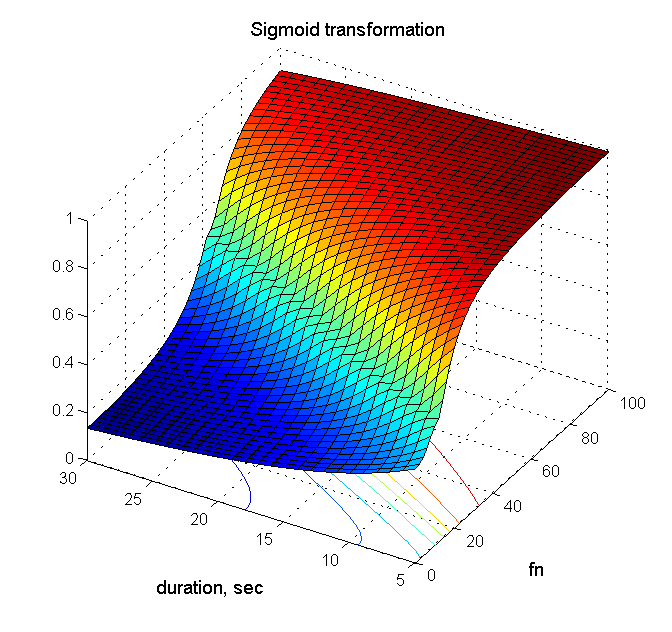
\includegraphics
			[width=.49\textwidth,height=.9\textheight,keepaspectratio]
			{sigmoid.png}%
			\label{fig:sigmoid}}
	\end{figure}
\end{frame}

\begin{frame}	
	\frametitle{Rating}
	\begin{figure}[!t]
		\centering
		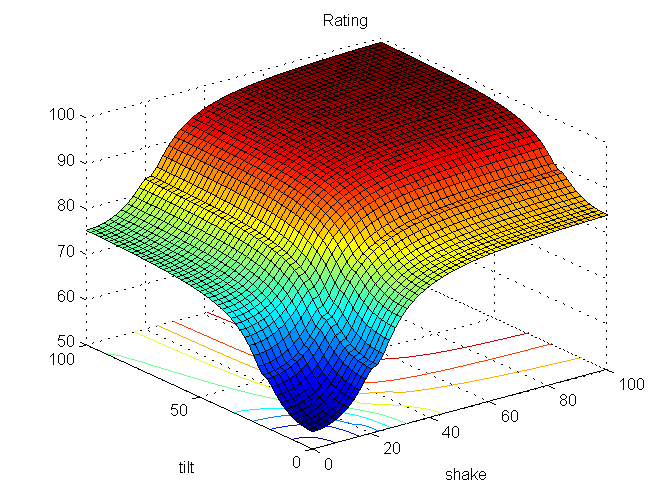
\includegraphics[width=\textwidth,height=.9\textheight,keepaspectratio]{rating.png}
		\label{fig:rating}
	\end{figure}
\end{frame}